% Options for packages loaded elsewhere
\PassOptionsToPackage{unicode}{hyperref}
\PassOptionsToPackage{hyphens}{url}
\PassOptionsToPackage{dvipsnames,svgnames,x11names}{xcolor}
%
\documentclass[
  letterpaper,
  DIV=11,
  numbers=noendperiod]{scrartcl}

\usepackage{amsmath,amssymb}
\usepackage{iftex}
\ifPDFTeX
  \usepackage[T1]{fontenc}
  \usepackage[utf8]{inputenc}
  \usepackage{textcomp} % provide euro and other symbols
\else % if luatex or xetex
  \usepackage{unicode-math}
  \defaultfontfeatures{Scale=MatchLowercase}
  \defaultfontfeatures[\rmfamily]{Ligatures=TeX,Scale=1}
\fi
\usepackage{lmodern}
\ifPDFTeX\else  
    % xetex/luatex font selection
\fi
% Use upquote if available, for straight quotes in verbatim environments
\IfFileExists{upquote.sty}{\usepackage{upquote}}{}
\IfFileExists{microtype.sty}{% use microtype if available
  \usepackage[]{microtype}
  \UseMicrotypeSet[protrusion]{basicmath} % disable protrusion for tt fonts
}{}
\makeatletter
\@ifundefined{KOMAClassName}{% if non-KOMA class
  \IfFileExists{parskip.sty}{%
    \usepackage{parskip}
  }{% else
    \setlength{\parindent}{0pt}
    \setlength{\parskip}{6pt plus 2pt minus 1pt}}
}{% if KOMA class
  \KOMAoptions{parskip=half}}
\makeatother
\usepackage{xcolor}
\setlength{\emergencystretch}{3em} % prevent overfull lines
\setcounter{secnumdepth}{5}
% Make \paragraph and \subparagraph free-standing
\ifx\paragraph\undefined\else
  \let\oldparagraph\paragraph
  \renewcommand{\paragraph}[1]{\oldparagraph{#1}\mbox{}}
\fi
\ifx\subparagraph\undefined\else
  \let\oldsubparagraph\subparagraph
  \renewcommand{\subparagraph}[1]{\oldsubparagraph{#1}\mbox{}}
\fi


\providecommand{\tightlist}{%
  \setlength{\itemsep}{0pt}\setlength{\parskip}{0pt}}\usepackage{longtable,booktabs,array}
\usepackage{calc} % for calculating minipage widths
% Correct order of tables after \paragraph or \subparagraph
\usepackage{etoolbox}
\makeatletter
\patchcmd\longtable{\par}{\if@noskipsec\mbox{}\fi\par}{}{}
\makeatother
% Allow footnotes in longtable head/foot
\IfFileExists{footnotehyper.sty}{\usepackage{footnotehyper}}{\usepackage{footnote}}
\makesavenoteenv{longtable}
\usepackage{graphicx}
\makeatletter
\def\maxwidth{\ifdim\Gin@nat@width>\linewidth\linewidth\else\Gin@nat@width\fi}
\def\maxheight{\ifdim\Gin@nat@height>\textheight\textheight\else\Gin@nat@height\fi}
\makeatother
% Scale images if necessary, so that they will not overflow the page
% margins by default, and it is still possible to overwrite the defaults
% using explicit options in \includegraphics[width, height, ...]{}
\setkeys{Gin}{width=\maxwidth,height=\maxheight,keepaspectratio}
% Set default figure placement to htbp
\makeatletter
\def\fps@figure{htbp}
\makeatother
\newlength{\cslhangindent}
\setlength{\cslhangindent}{1.5em}
\newlength{\csllabelwidth}
\setlength{\csllabelwidth}{3em}
\newlength{\cslentryspacingunit} % times entry-spacing
\setlength{\cslentryspacingunit}{\parskip}
\newenvironment{CSLReferences}[2] % #1 hanging-ident, #2 entry spacing
 {% don't indent paragraphs
  \setlength{\parindent}{0pt}
  % turn on hanging indent if param 1 is 1
  \ifodd #1
  \let\oldpar\par
  \def\par{\hangindent=\cslhangindent\oldpar}
  \fi
  % set entry spacing
  \setlength{\parskip}{#2\cslentryspacingunit}
 }%
 {}
\usepackage{calc}
\newcommand{\CSLBlock}[1]{#1\hfill\break}
\newcommand{\CSLLeftMargin}[1]{\parbox[t]{\csllabelwidth}{#1}}
\newcommand{\CSLRightInline}[1]{\parbox[t]{\linewidth - \csllabelwidth}{#1}\break}
\newcommand{\CSLIndent}[1]{\hspace{\cslhangindent}#1}

\usepackage{float}
\usepackage{tabularray}
\usepackage[normalem]{ulem}
\usepackage{graphicx}
\UseTblrLibrary{booktabs}
\UseTblrLibrary{siunitx}
\NewTableCommand{\tinytableDefineColor}[3]{\definecolor{#1}{#2}{#3}}
\newcommand{\tinytableTabularrayUnderline}[1]{\underline{#1}}
\newcommand{\tinytableTabularrayStrikeout}[1]{\sout{#1}}
\KOMAoption{captions}{tableheading}
\makeatletter
\makeatother
\makeatletter
\makeatother
\makeatletter
\@ifpackageloaded{caption}{}{\usepackage{caption}}
\AtBeginDocument{%
\ifdefined\contentsname
  \renewcommand*\contentsname{Table of contents}
\else
  \newcommand\contentsname{Table of contents}
\fi
\ifdefined\listfigurename
  \renewcommand*\listfigurename{List of Figures}
\else
  \newcommand\listfigurename{List of Figures}
\fi
\ifdefined\listtablename
  \renewcommand*\listtablename{List of Tables}
\else
  \newcommand\listtablename{List of Tables}
\fi
\ifdefined\figurename
  \renewcommand*\figurename{Figure}
\else
  \newcommand\figurename{Figure}
\fi
\ifdefined\tablename
  \renewcommand*\tablename{Table}
\else
  \newcommand\tablename{Table}
\fi
}
\@ifpackageloaded{float}{}{\usepackage{float}}
\floatstyle{ruled}
\@ifundefined{c@chapter}{\newfloat{codelisting}{h}{lop}}{\newfloat{codelisting}{h}{lop}[chapter]}
\floatname{codelisting}{Listing}
\newcommand*\listoflistings{\listof{codelisting}{List of Listings}}
\makeatother
\makeatletter
\@ifpackageloaded{caption}{}{\usepackage{caption}}
\@ifpackageloaded{subcaption}{}{\usepackage{subcaption}}
\makeatother
\makeatletter
\@ifpackageloaded{tcolorbox}{}{\usepackage[skins,breakable]{tcolorbox}}
\makeatother
\makeatletter
\@ifundefined{shadecolor}{\definecolor{shadecolor}{rgb}{.97, .97, .97}}
\makeatother
\makeatletter
\makeatother
\makeatletter
\makeatother
\ifLuaTeX
  \usepackage{selnolig}  % disable illegal ligatures
\fi
\IfFileExists{bookmark.sty}{\usepackage{bookmark}}{\usepackage{hyperref}}
\IfFileExists{xurl.sty}{\usepackage{xurl}}{} % add URL line breaks if available
\urlstyle{same} % disable monospaced font for URLs
\hypersetup{
  pdftitle={My title},
  pdfauthor={Sandy Yu},
  colorlinks=true,
  linkcolor={blue},
  filecolor={Maroon},
  citecolor={Blue},
  urlcolor={Blue},
  pdfcreator={LaTeX via pandoc}}

\title{My title\thanks{Code and data are available at:
https://github.com/Jingying-yu/Shanghai\_population\_change}}
\usepackage{etoolbox}
\makeatletter
\providecommand{\subtitle}[1]{% add subtitle to \maketitle
  \apptocmd{\@title}{\par {\large #1 \par}}{}{}
}
\makeatother
\subtitle{Impact Analysis of Japanese Occupation on Population Shifts
Across Shanghai's Districts During WWII}
\author{Sandy Yu}
\date{November 30, 2024}

\begin{document}
\maketitle
\begin{abstract}
First sentence. Second sentence. Third sentence. Fourth sentence.
\end{abstract}
\ifdefined\Shaded\renewenvironment{Shaded}{\begin{tcolorbox}[enhanced, breakable, frame hidden, boxrule=0pt, interior hidden, borderline west={3pt}{0pt}{shadecolor}, sharp corners]}{\end{tcolorbox}}\fi

\hypertarget{introduction}{%
\section{Introduction}\label{introduction}}

Overview paragraph

Estimand paragraph

Results paragraph

Why it matters paragraph

Telegraphing paragraph: The remainder of this paper is structured as
follows. Section~\ref{sec-data}\ldots.

\hypertarget{sec-data}{%
\section{Data}\label{sec-data}}

\hypertarget{overview}{%
\subsection{Overview}\label{overview}}

We use the statistical programming language R (R Core Team 2023)\ldots.
Our data (Toronto Shelter \& Support Services 2024)\ldots. Following
Alexander (2023), we consider\ldots{}

\hypertarget{data-sources}{%
\subsection{Data Sources}\label{data-sources}}

\begin{itemize}
\tightlist
\item
  talk about where the data in my primary reference book is gathered
\item
  mentions the credibility of source and unstability of recording
  instrument \& methodology
\end{itemize}

\hypertarget{historical-background}{%
\subsection{Historical Background}\label{historical-background}}

Place: Shanghai, China When: 1936-1942 Who: Chinese population in
Shanghai

Define: 1. give 1-2 sentence broad overview of China's state of unrest
2.THREE districts in Shanghai: Chinese District, International
Settlement, French Concession - who controlled each district and the
level of governance each authority have in comparison to Chinese
government 3.Outline area (\%) of each district (do not get into
specifics, put that in Results section)

Important Event Timeline 1. 1937-08-13: Japanese armed forces entered
Shanghai 2. 1937-11-12: Japanese armed forces claims occupation of
Shanghai --\textgreater{} ends Chinese district 3. 1942-01: Japanese
armed forces claims authority over International Settlement (which was
mainly under the governance of U.K and U.S prior to this date) 4.
1945-08-15: Japan surrendered in WWII 5. 1945-10: most Japanese armed
forces withdrawed from Shanghai

\hypertarget{measurement}{%
\subsection{Measurement}\label{measurement}}

\begin{itemize}
\tightlist
\item
  how population is recorded (not accurate count but by householad then
  estimates by average)
\item
  why use population density instead of pure population \#
\item
  how year variables correspond to the timeline (ex. if an event occured
  in Nov of 1937, would I take valeus of 1937 as a variable for prior to
  event occurance or after?)
\end{itemize}

\hypertarget{outcome-variables}{%
\subsection{Outcome variables}\label{outcome-variables}}

\begin{itemize}
\tightlist
\item
  outcome variable is ``population change in International Settlement
  during 1937-1942'' measured in population density
\end{itemize}

\hypertarget{predictor-variables}{%
\subsection{Predictor variables}\label{predictor-variables}}

\begin{itemize}
\tightlist
\item
  most important predictors include time sensitive indicators: Event1 \&
  Event2
\end{itemize}

Event1: indicator variable for 1937 (1 if year \textgreater= 1937 \&
\textless= 1941, 0 otherwise) - mention a bit about the measurement

Event2: indicator variable for 1937 (1 if year \textgreater= 1941, 0
otherwise) - mention a bit about the measurement

\hypertarget{model}{%
\section{Model}\label{model}}

The goal of our modelling strategy is to evaluate the impact of 2
historical events in Shanghai during WWII.

Here we briefly describe the Difference-in-Difference analysis model
used to investigate the impact of the Japanese forces taking over the
Chinese district and International Settlement in November 1937 and
December 1941 on population shift between different Districts in
Shanghai.

Background details and diagnostics are included in
Appendix~\ref{sec-model-details}.

\hypertarget{model-set-up}{%
\subsection{Model set-up}\label{model-set-up}}

\[y_{it}|\mu_{it}, \sigma \sim \mbox{Normal}(\mu_{it}, \sigma)\]

\[\mu_{it} = \alpha + \beta_1 \cdot \mbox{cd_occupied}_{it} + \beta_2 \cdot \mbox{french_surrender}_{it} + \beta_3 \cdot \mbox{is_occupied}_{it} + \beta_4 \cdot \mbox{district_type}_{i, IS} +
\\
\beta_5 \cdot \mbox{district_type}_{i, FC} + \beta_6 \cdot \mbox{cd_occupied}_{it} \cdot \mbox{district_type}_{i, IS} + 
\\
\beta_7 \cdot \mbox{cd_occupied}_{it} \cdot \mbox{district_type}_{i, FC} + \beta_8 \cdot \mbox{french_surrender}_{it} \cdot \mbox{district_type}_{i, IS} + 
\\
\beta_9 \cdot \mbox{french_surrender}_{it} \cdot \mbox{district_type}_{i, FC} + 
\\
\beta_{10} \cdot \mbox{is_occupied}_{it} \cdot \mbox{district_type}_{i, IS} + \beta_{11} \cdot \mbox{is_occupied}_{it} \cdot \mbox{district_type}_{i, FC}\]

\[\alpha \sim \mbox{Normal}(0, 2.5)\]

\[\beta_k \sim \mbox{Normal}(0, 2.5) \quad \mbox{for } k = 1, ..., 11\]

\[\sigma \sim \mbox{Exponential}(1)\]

\textbf{Where}:

\begin{itemize}
\tightlist
\item
  \(y_{i,t}\): Observed population in district i at year t.
\item
  \(\mbox{cd_occupied}_{i,t}\): Indicator for whether the
  Chinese-administered district was occupied by Japanese forces in year
  t (1 if \(t \geq 1937\), 0 otherwise).
\item
  \(\mbox{french_surrender}_{i,t}\): Indicator for the French
  Surrendering to Germany in 1940, leading to the French Concession
  rejecting refugees in Shanghai (1 if \(t \geq 1940\), 0 otherwise).
\item
  \(\mbox{is_occupied}_{i,t}\): Indicator for the Japanese occupation of
  the International Settlement in 1942 (1 if \(t \geq 1942\), 0
  otherwise).
\item
  \(\mbox{district_type}_{i, IS}\): Dummy variable for International
  Settlement districts (1 if i is IS, 0 otherwise).
\item
  \(\mbox{district_type}_{i, FC}\): Dummy variable for French Concession
  districts (1 if i is FC, 0 otherwise).
\end{itemize}

\textbf{Interaction Terms}: The interaction terms in the model are
essential because they capture how the impact of historical events
(e.g., the 1937 occupation of Chinese-administered districts, the 1940
refugee rejection in the French Concession, and the 1942 occupation of
the International Settlement) varies across different district types. By
including interactions between event indicators and district types, the
model accounts for district-specific responses to each event,
controlling for the fact that the effect of an event on population
changes may not be uniform across all districts. For instance, the 1937
occupation might lead to population declines in Chinese-administered
districts but population increases in the International Settlement due
to refugee influx. These terms ensure that the model can differentiate
and estimate the unique effects of each event within each district type,
thereby improving precision and interpretability.

\begin{itemize}
\tightlist
\item
  \(\mbox{cd_occupied}_{i,t} \cdot \mbox{district_type}_{i, IS}\):
  Captures the effect of the 1937 occupation on the International
  Settlement in comparison to the Chinese-administered district (base
  district).
\item
  \(\mbox{cd_occupied}_{i,t} \cdot \mbox{district_type}_{i, FC}\):
  Captures the effect of the 1937 occupation on the French Concession in
  comparison to the base district.
\item
  \(\mbox{french_surrender}_{i,t} \cdot \mbox{district_type}_{i, IS}\):
  Effect of the 1940 refugee rejection on the International Settlement.
\item
  \(\mbox{french_surrender}_{i,t} \cdot \mbox{district_type}_{i, FC}\):
  Effect of the 1940 refugee rejection on the French Concession.
\item
  \(\mbox{is_occupied}_{i,t} \cdot \mbox{district_type}_{i, IS}\):
  Effect of the 1942 occupation on the International Settlement.
\item
  \(\mbox{is_occupied}_{i,t} \cdot \mbox{district_type}_{i, FC}\):
  Effect of the 1942 occupation on the French Concession.
\end{itemize}

We run the model in R (R Core Team 2023) using the \texttt{rstanarm}
package of Goodrich et al. (2022). We use the default priors from
\texttt{rstanarm}.

\hypertarget{model-justification}{%
\subsubsection{Model justification}\label{model-justification}}

We expect a positive relationship between the size of the wings and time
spent aloft. In particular\ldots{}

We can use maths by including latex between dollar signs, for instance
\(\theta\).

\hypertarget{results}{%
\section{Results}\label{results}}

Our results are summarized in Table~\ref{tbl-modelresults}.

\hypertarget{tbl-modelresults}{}
\begin{table}
\caption{\label{tbl-modelresults}Explanatory models of flight time based on wing width and wing length }\tabularnewline

\centering
\begin{tblr}[         %% tabularray outer open
]                     %% tabularray outer close
{                     %% tabularray inner open
colspec={Q[]Q[]},
column{1}={halign=l,},
column{2}={halign=c,},
hline{26}={1,2}{solid, 0.05em, black},
}                     %% tabularray inner close
\toprule
& Population model \\ \midrule %% TinyTableHeader
(Intercept)                                                  & \num{-0.05}      \\
& (\num{15.64})    \\
cd\_occupied                                                & \num{0.15}       \\
& (\num{10.22})    \\
district\_typeFrench Concession                             & \num{-0.11}      \\
& (\num{9.98})     \\
district\_typeInternational Settlement                      & \num{0.07}       \\
& (\num{9.83})     \\
french\_surrender                                           & \num{-0.06}      \\
& (\num{10.22})    \\
is\_occupied                                                & \num{-0.17}      \\
& (\num{9.95})     \\
cd\_occupied × district\_typeFrench Concession             & \num{-0.07}      \\
& (\num{9.95})     \\
cd\_occupied × district\_typeInternational Settlement      & \num{-0.06}      \\
& (\num{9.81})     \\
district\_typeFrench Concession × french\_surrender        & \num{0.01}       \\
& (\num{9.96})     \\
district\_typeInternational Settlement × french\_surrender & \num{-0.02}      \\
& (\num{10.01})    \\
district\_typeFrench Concession × is\_occupied             & \num{0.01}       \\
& (\num{10.20})    \\
district\_typeInternational Settlement × is\_occupied      & \num{0.00}       \\
& (\num{9.85})     \\
Num.Obs.                                                     & \num{21}         \\
R2                                                           & \num{0.000}      \\
Log.Lik.                                                     & \num{-325.376}   \\
RMSE                                                         & \num{1293540.34} \\
\bottomrule
\end{tblr}
\end{table}

\hypertarget{discussion}{%
\section{Discussion}\label{discussion}}

\hypertarget{reason-why-the-french-concession-was-exempted-from-japanese-occupation}{%
\subsection{Reason why the French Concession was Exempted from Japanese
Occupation}\label{reason-why-the-french-concession-was-exempted-from-japanese-occupation}}

\begin{itemize}
\tightlist
\item
  During WWII, on the European battlefield, France surrendered to
  Germany on June 22nd of 1940 (Check this \& reference with a credible
  source). Since Japan was on the same side as Germany during that time,
  Japanese armed forces decided allow the French Concession to retain
  its own governance.
\item
  However, the French Concession is still constantly under the watch of
  the Japanese forces that has occupied the rest of Shanghai since 1942.
  街上不得有侮辱日本的旗帜或者宣言,官方必须积极配合日本统治者进行有利于日本统治的宣传,etc.(can
  reference to video summary here)
\end{itemize}

\hypertarget{refugees-from-outside-of-shanghai-province}{%
\subsection{Refugees from outside of Shanghai
Province}\label{refugees-from-outside-of-shanghai-province}}

\begin{itemize}
\tightlist
\item
  industrialization was not so popular back in the 1930s, many provinces
  are still mostly rural. But warfare messed with the land and the
  yields, causing many farmers to starve and ultimately have to seek
  refugee (find job) in industrialized city (where income is not
  dependent on land yield)
\item
  many people flooded to Shanghai for this reason (can insert
  calculation in data table 20 from reference book here)
\end{itemize}

\hypertarget{job-oppurtunities-in-shanghai}{%
\subsubsection{Job Oppurtunities in
Shanghai}\label{job-oppurtunities-in-shanghai}}

Aside from the instability caused by the Japanese armed forces, there
are a few other reasons for Chinese population to move into the
international settlement \& French Concession. 1. Job opportunities -
Heart of Shanghai city in the 1930-1940s, high pop density lead to boom
of economy = more job opportunities - many factories are located with
the settlements (less so in concession)

\hypertarget{barrier-to-entry-in-job-market}{%
\subsubsection{Barrier to Entry in Job
Market}\label{barrier-to-entry-in-job-market}}

\begin{enumerate}
\def\labelenumi{\arabic{enumi}.}
\setcounter{enumi}{1}
\tightlist
\item
  Barrier to Entry for certain job types
\end{enumerate}

\begin{itemize}
\tightlist
\item
  旧时候 --
  通讯还没有那么发达的时候,人们都很团结。那个时候同乡会的力量很强大。在外省,从同一个省来的漂泊者会互相帮扶着垄断一个城市的某种行业。例如,在旧上海,要做酒店生意的话你就必须是湖南人,给人做洗脚生意的肯定是苏北人。。。
\end{itemize}

\hypertarget{instability-after-japanese-occupation-ends-in-wwii-chinese-civil-war}{%
\subsection{Instability after Japanese Occupation ends in WWII: Chinese
Civil
War}\label{instability-after-japanese-occupation-ends-in-wwii-chinese-civil-war}}

\begin{itemize}
\tightlist
\item
  after the Japanese armed forces withdrawed from Shanghai, what follows
  is not recovery and rest for the local population
\item
  Competition for power within China's 2 political parties caused
  full-scale political warfare, now known as the \emph{Chinese Civil
  War}
\item
  unlike Western political parties, Chinese political parties in the
  1900s are more like parties of a throne. They each have their own
  ideology and an armed forces that follow. Most of all of the provinces
  are effected by this internal warfare, which ended in 1949 as 国民党
  lost and withdrawed to Taiwan.
\end{itemize}

\hypertarget{weaknesses-and-next-steps}{%
\subsection{Weaknesses and next steps}\label{weaknesses-and-next-steps}}

\hypertarget{data-measurement-weaknesses}{%
\subsubsection{Data Measurement
Weaknesses}\label{data-measurement-weaknesses}}

\begin{itemize}
\tightlist
\item
  data was recorded during wartime, many numbers were missing
\item
  base unit for population records is not ppl, it is instead
  ``household''. \# of ppl in a household is estimated based on
  historical data
\item
  many people chose to not report or partially report numbers due to
  convience or economic reasons, data may not be accurate
\end{itemize}

\hypertarget{next-steps}{%
\subsubsection{Next Steps}\label{next-steps}}

\newpage

\appendix

\hypertarget{appendix}{%
\section*{Appendix}\label{appendix}}
\addcontentsline{toc}{section}{Appendix}

\hypertarget{additional-data-details}{%
\section{Additional data details}\label{additional-data-details}}

\hypertarget{sec-model-details}{%
\section{Model details}\label{sec-model-details}}

\hypertarget{posterior-predictive-check}{%
\subsection{Posterior predictive
check}\label{posterior-predictive-check}}

In Figure~\ref{fig-ppcheckandposteriorvsprior-1} we implement a
posterior predictive check. This shows\ldots{}

In Figure~\ref{fig-ppcheckandposteriorvsprior-2} we compare the
posterior with the prior. This shows\ldots{}

\begin{figure}

\begin{minipage}[t]{0.50\linewidth}

{\centering 

\raisebox{-\height}{

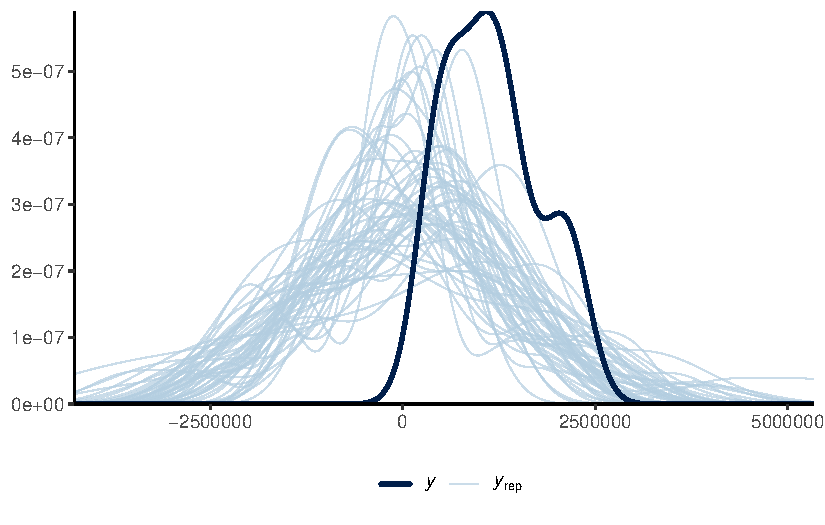
\includegraphics{paper_files/figure-pdf/fig-ppcheckandposteriorvsprior-1.pdf}

}

}

\subcaption{\label{fig-ppcheckandposteriorvsprior-1}Posterior prediction
check}
\end{minipage}%
%
\begin{minipage}[t]{0.50\linewidth}

{\centering 

\raisebox{-\height}{

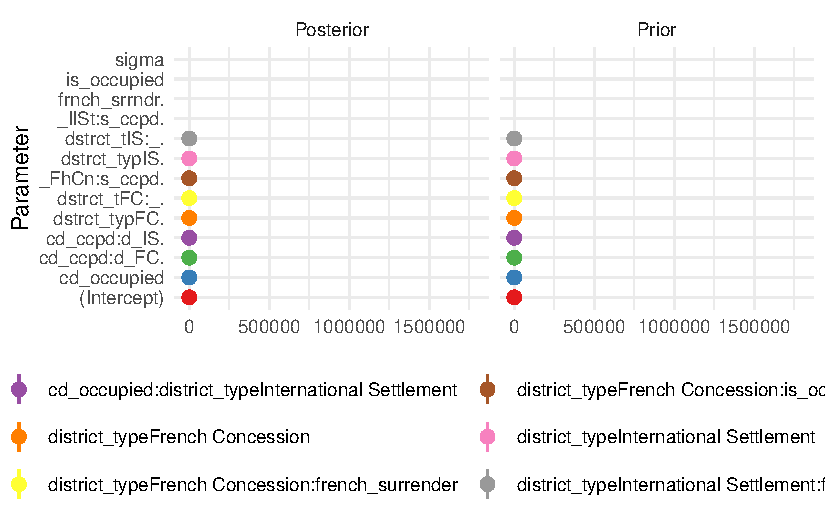
\includegraphics{paper_files/figure-pdf/fig-ppcheckandposteriorvsprior-2.pdf}

}

}

\subcaption{\label{fig-ppcheckandposteriorvsprior-2}Comparing the
posterior with the prior}
\end{minipage}%

\caption{\label{fig-ppcheckandposteriorvsprior}Examining how the model
fits, and is affected by, the data}

\end{figure}

\hypertarget{diagnostics}{%
\subsection{Diagnostics}\label{diagnostics}}

Figure~\ref{fig-stanareyouokay-1} is a trace plot. It shows\ldots{} This
suggests\ldots{}

Figure~\ref{fig-stanareyouokay-2} is a Rhat plot. It shows\ldots{} This
suggests\ldots{}

\begin{figure}

\begin{minipage}[t]{0.50\linewidth}

{\centering 

\raisebox{-\height}{

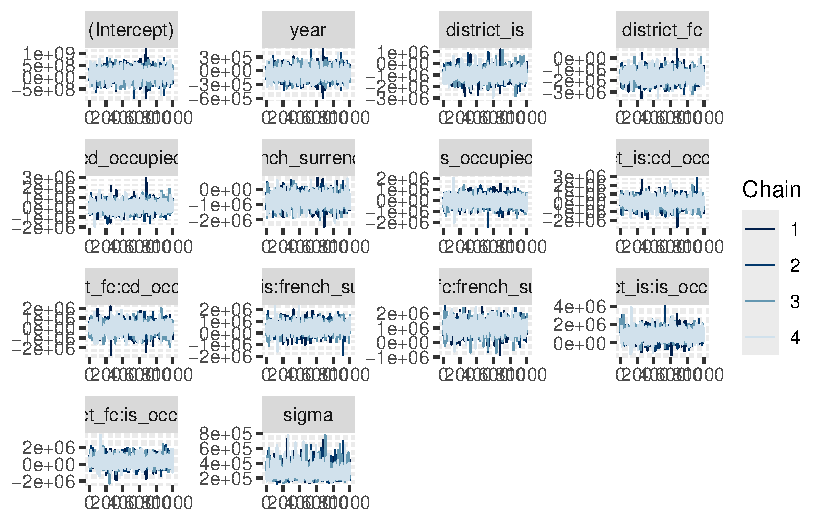
\includegraphics{paper_files/figure-pdf/fig-stanareyouokay-1.pdf}

}

}

\subcaption{\label{fig-stanareyouokay-1}Trace plot}
\end{minipage}%
%
\begin{minipage}[t]{0.50\linewidth}

{\centering 

\raisebox{-\height}{

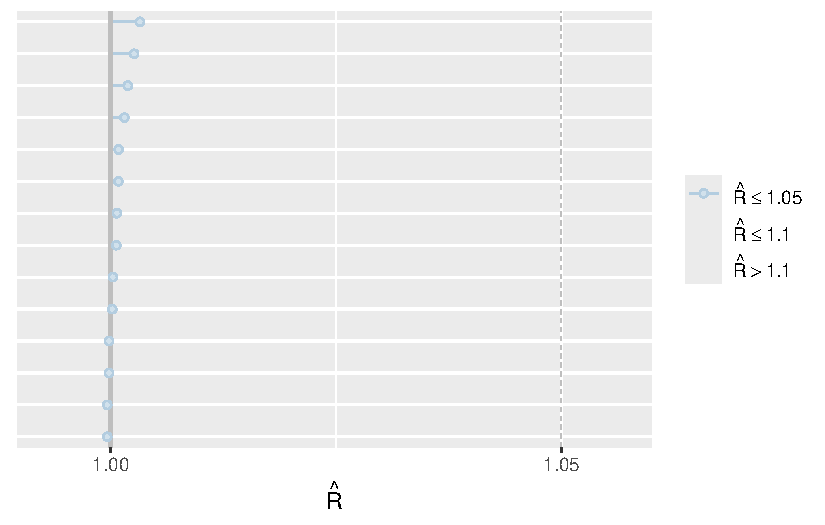
\includegraphics{paper_files/figure-pdf/fig-stanareyouokay-2.pdf}

}

}

\subcaption{\label{fig-stanareyouokay-2}Rhat plot}
\end{minipage}%

\caption{\label{fig-stanareyouokay}Checking the convergence of the MCMC
algorithm}

\end{figure}

\newpage

\hypertarget{references}{%
\section*{References}\label{references}}
\addcontentsline{toc}{section}{References}

\hypertarget{refs}{}
\begin{CSLReferences}{1}{0}
\leavevmode\vadjust pre{\hypertarget{ref-tellingstories}{}}%
Alexander, Rohan. 2023. \emph{Telling Stories with Data}. Chapman;
Hall/CRC. \url{https://tellingstorieswithdata.com/}.

\leavevmode\vadjust pre{\hypertarget{ref-rstanarm}{}}%
Goodrich, Ben, Jonah Gabry, Imad Ali, and Sam Brilleman. 2022.
{``{rstanarm: {Bayesian} applied regression modeling via {Stan}}.''}
\url{https://mc-stan.org/rstanarm/}.

\leavevmode\vadjust pre{\hypertarget{ref-citeR}{}}%
R Core Team. 2023. \emph{{R: A Language and Environment for Statistical
Computing}}. Vienna, Austria: R Foundation for Statistical Computing.
\url{https://www.R-project.org/}.

\leavevmode\vadjust pre{\hypertarget{ref-shelter}{}}%
Toronto Shelter \& Support Services. 2024. \emph{Deaths of Shelter
Residents}.
\url{https://open.toronto.ca/dataset/deaths-of-shelter-residents/}.

\end{CSLReferences}



\end{document}
